\subsection*{Transverse Momenta of \tauhadvis and $b$-Jet Candidates in the
  Signal Region}

\begin{figure}[htbp]
  \centering

  \begin{subfigure}{0.495\textwidth}
    \centering

    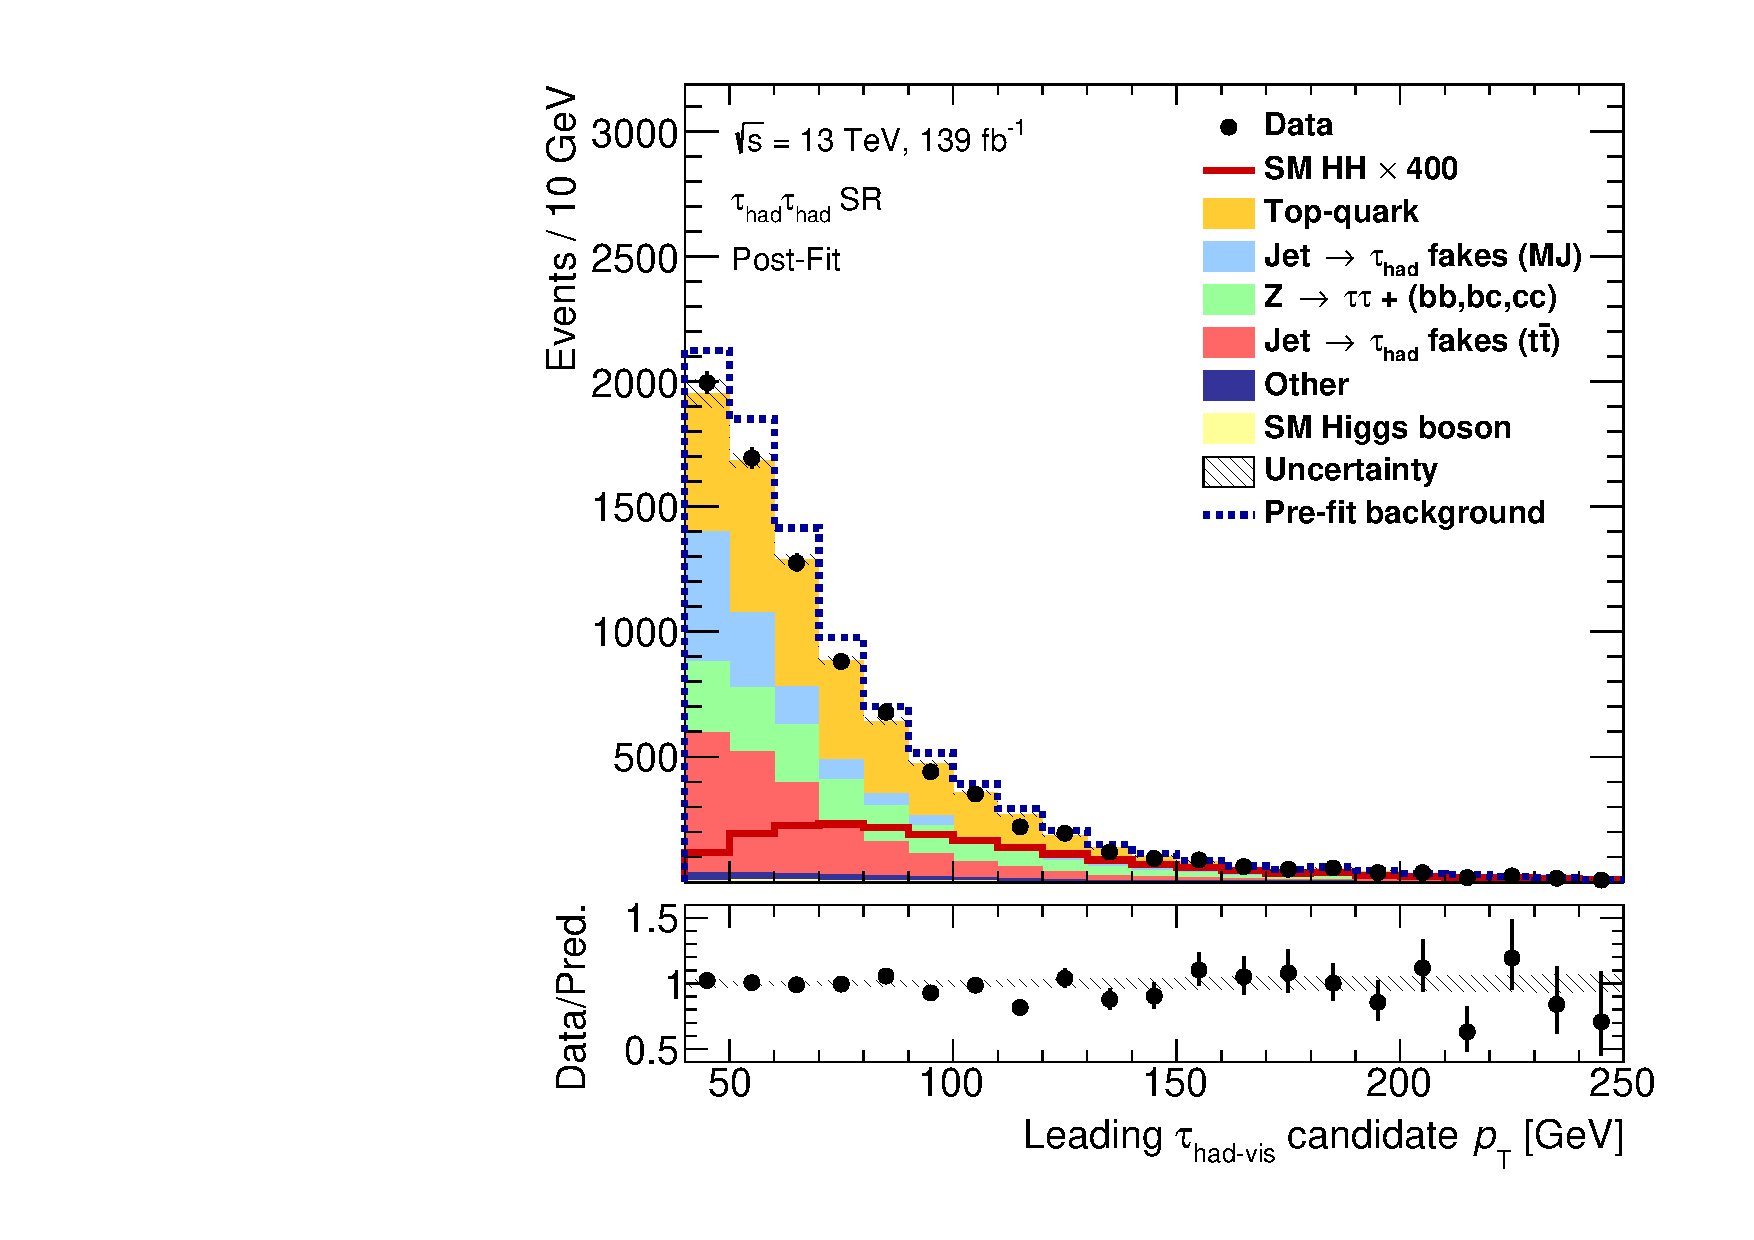
\includegraphics[width=\textwidth]{sr_postfit/Region_BMin0_incJet1_distTau0Pt_J2_Y2015_DLLOS_T2_SpcTauHH_L0_GlobalFit_conditionnal_mu0}
    \subcaption{}
  \end{subfigure}\hfill%
  \begin{subfigure}{0.495\textwidth}
    \centering

    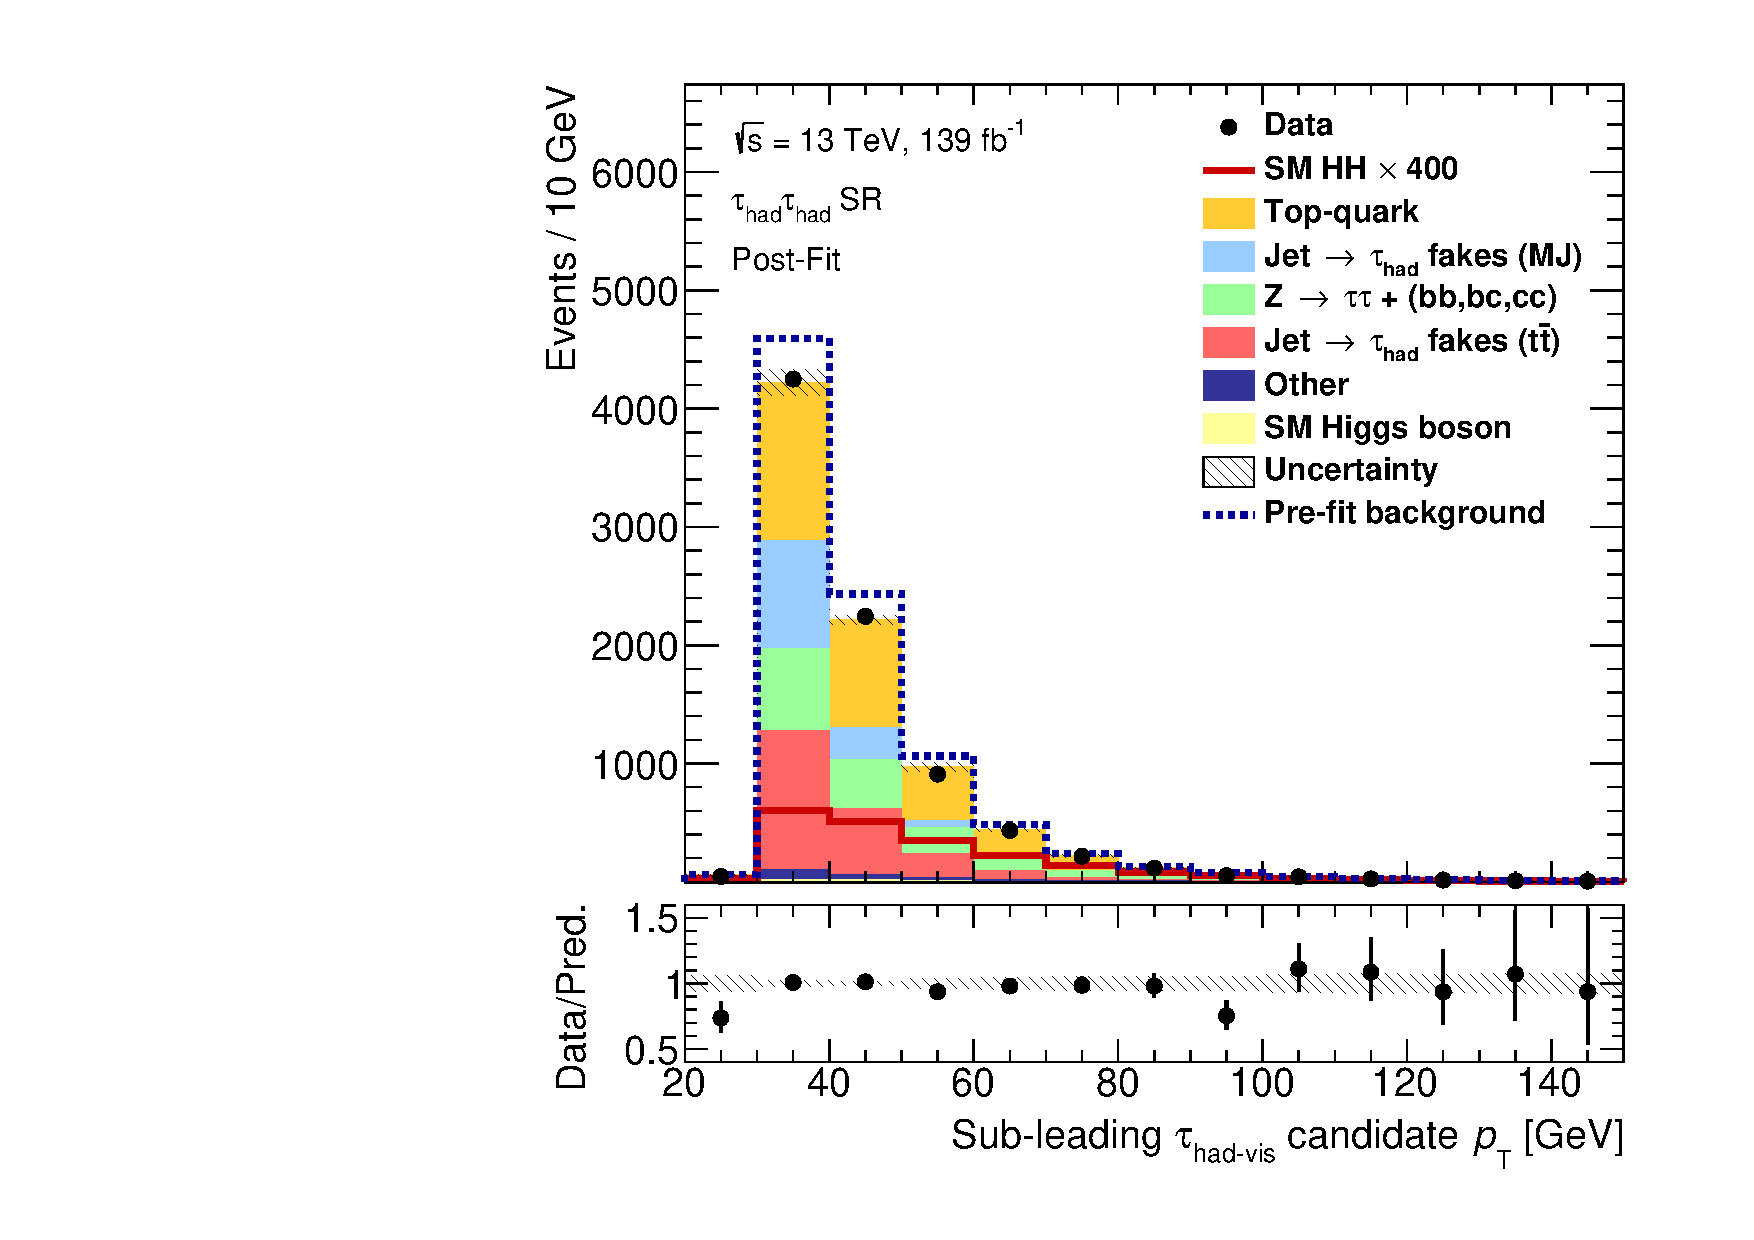
\includegraphics[width=\textwidth]{sr_postfit/Region_BMin0_incJet1_distTau1Pt_J2_Y2015_DLLOS_T2_SpcTauHH_L0_GlobalFit_conditionnal_mu0}
    \subcaption{}
  \end{subfigure}

  \begin{subfigure}{0.495\textwidth}
    \centering

    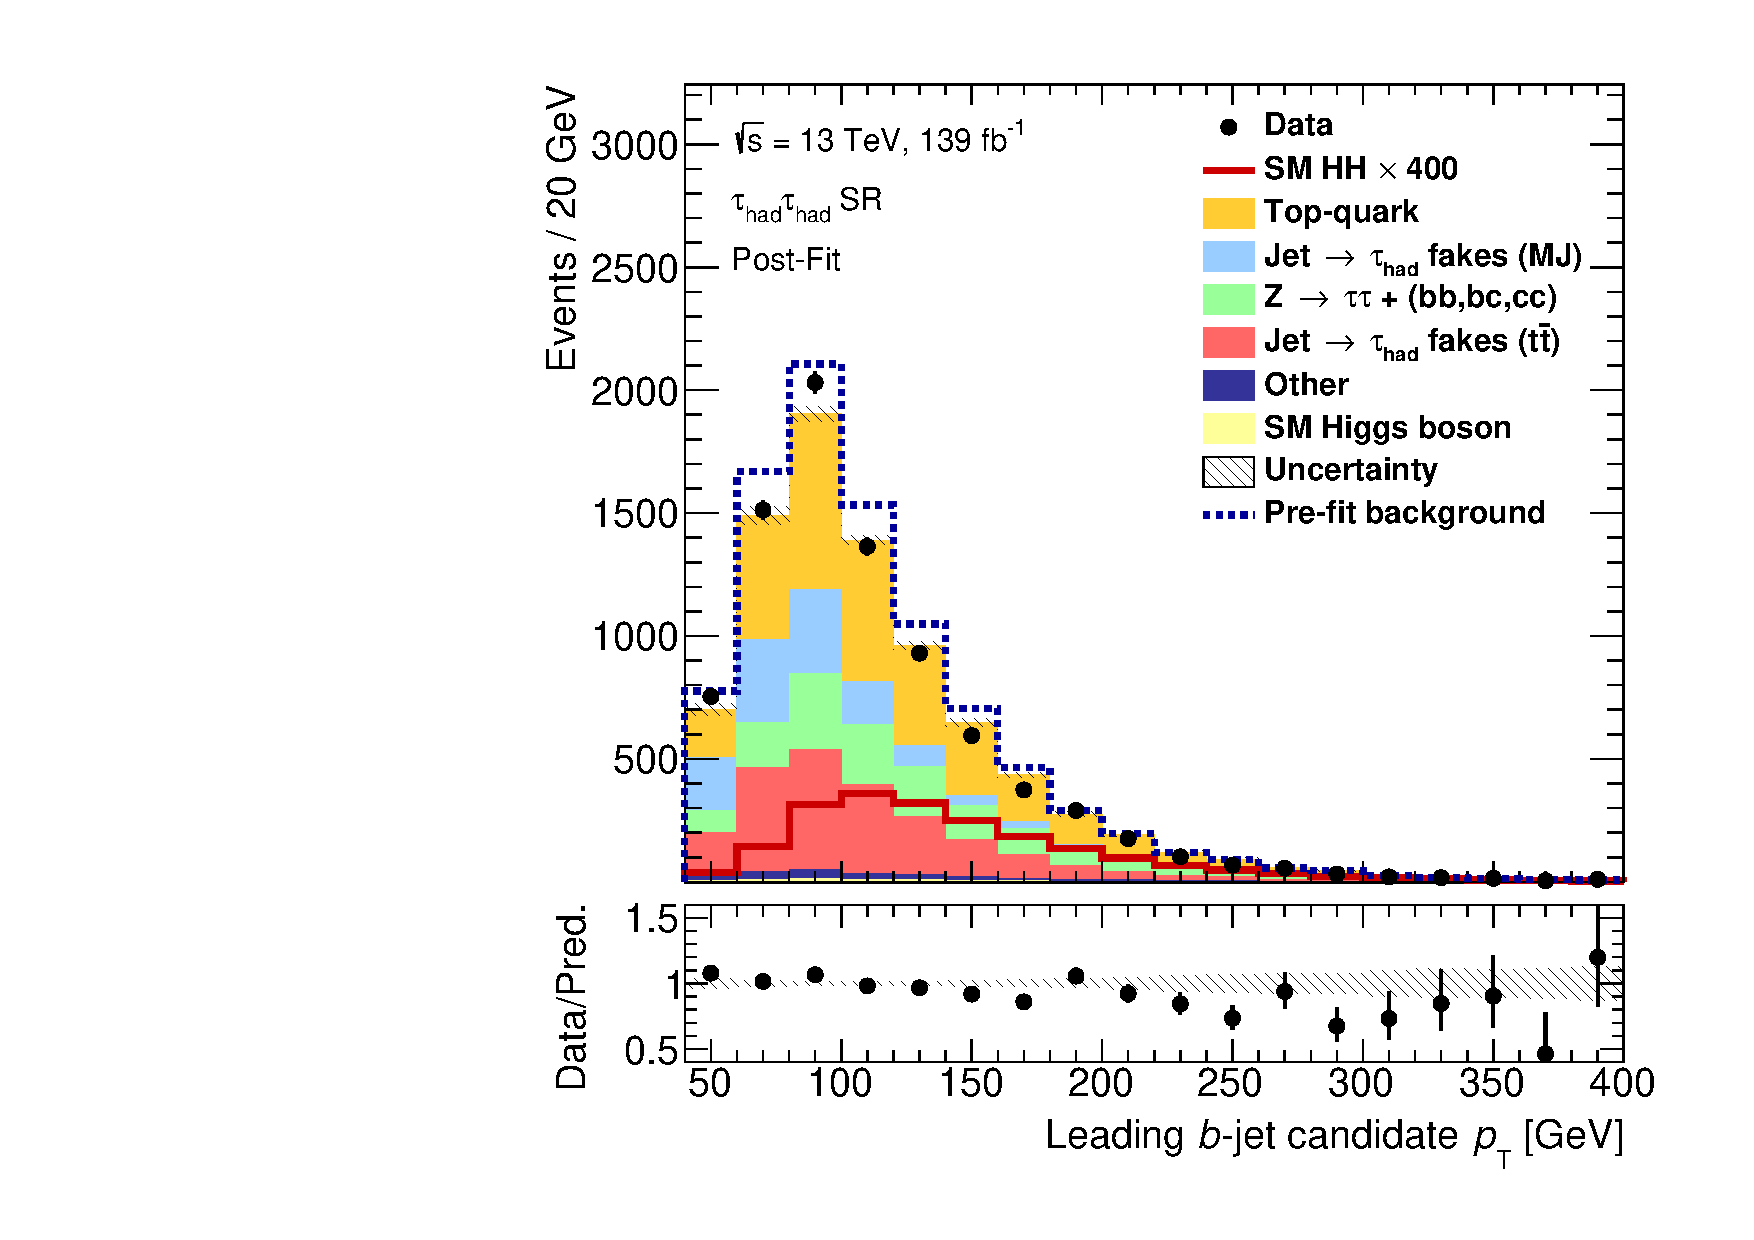
\includegraphics[width=\textwidth]{sr_postfit/Region_BMin0_incJet1_distpTB0_J2_Y2015_DLLOS_T2_SpcTauHH_L0_GlobalFit_conditionnal_mu0}
    \subcaption{}
  \end{subfigure}\hfill%
  \begin{subfigure}{0.495\textwidth}
    \centering

    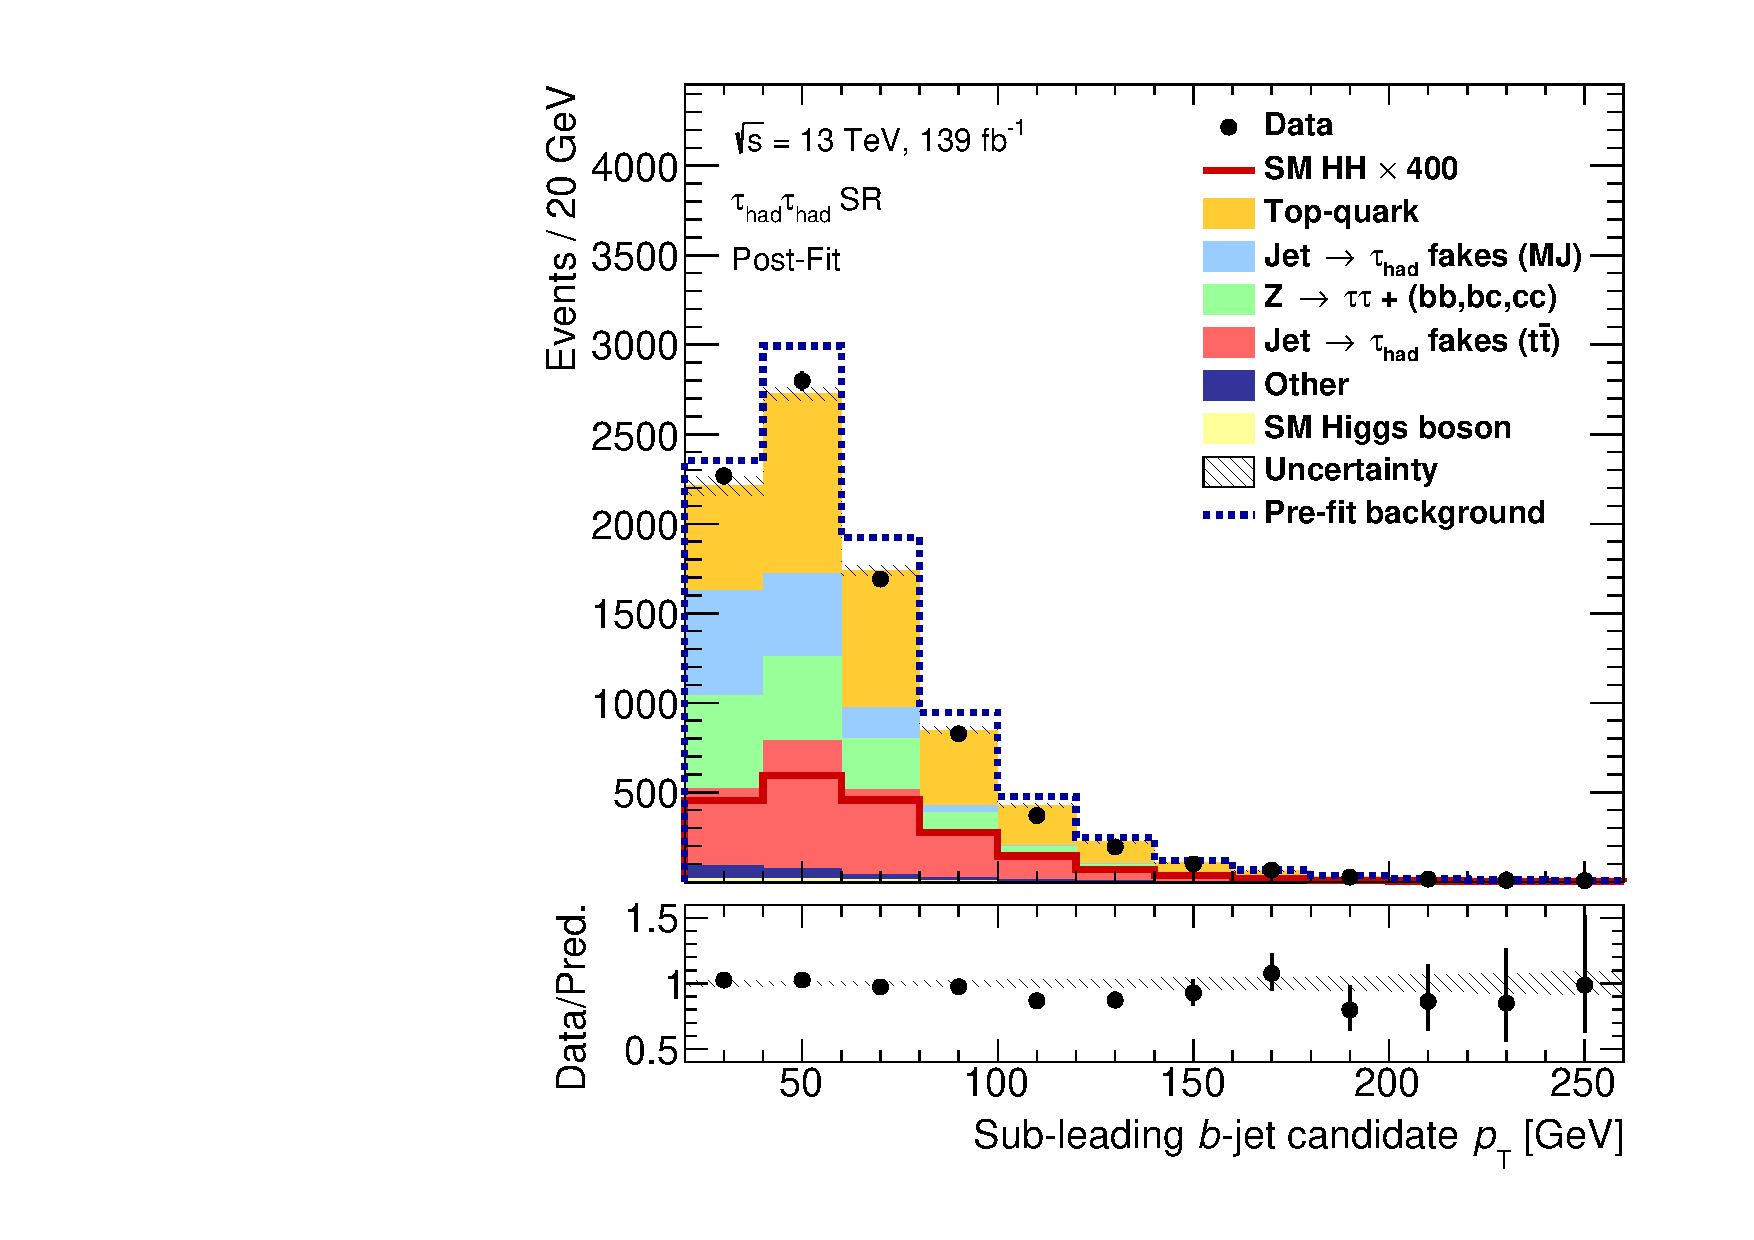
\includegraphics[width=\textwidth]{sr_postfit/Region_BMin0_incJet1_distpTB1_J2_Y2015_DLLOS_T2_SpcTauHH_L0_GlobalFit_conditionnal_mu0}
    \subcaption{}
  \end{subfigure}

  \caption[Distributions of the leading and sub-leading \tauhadvis candidate \pT
  and the leading and sub-leading $b$-jet candidate \pT in the SR of the \hadhad
  channel.]{Distributions of the leading and sub-leading \tauhadvis candidate
    \pT (a,b) and the leading and sub-leading $b$-jet candidate \pT (c,d) in the
    SR of the \hadhad channel after the background-only fit to data in all
    regions.}
\end{figure}


\clearpage
\subsection*{MVA Score Distributions in the \ZJets Validation Region}

{
  \centering

  \vspace*{1em}

  \setcaptiontype{figure}

  \begin{subfigure}{0.495\textwidth}
    \centering

    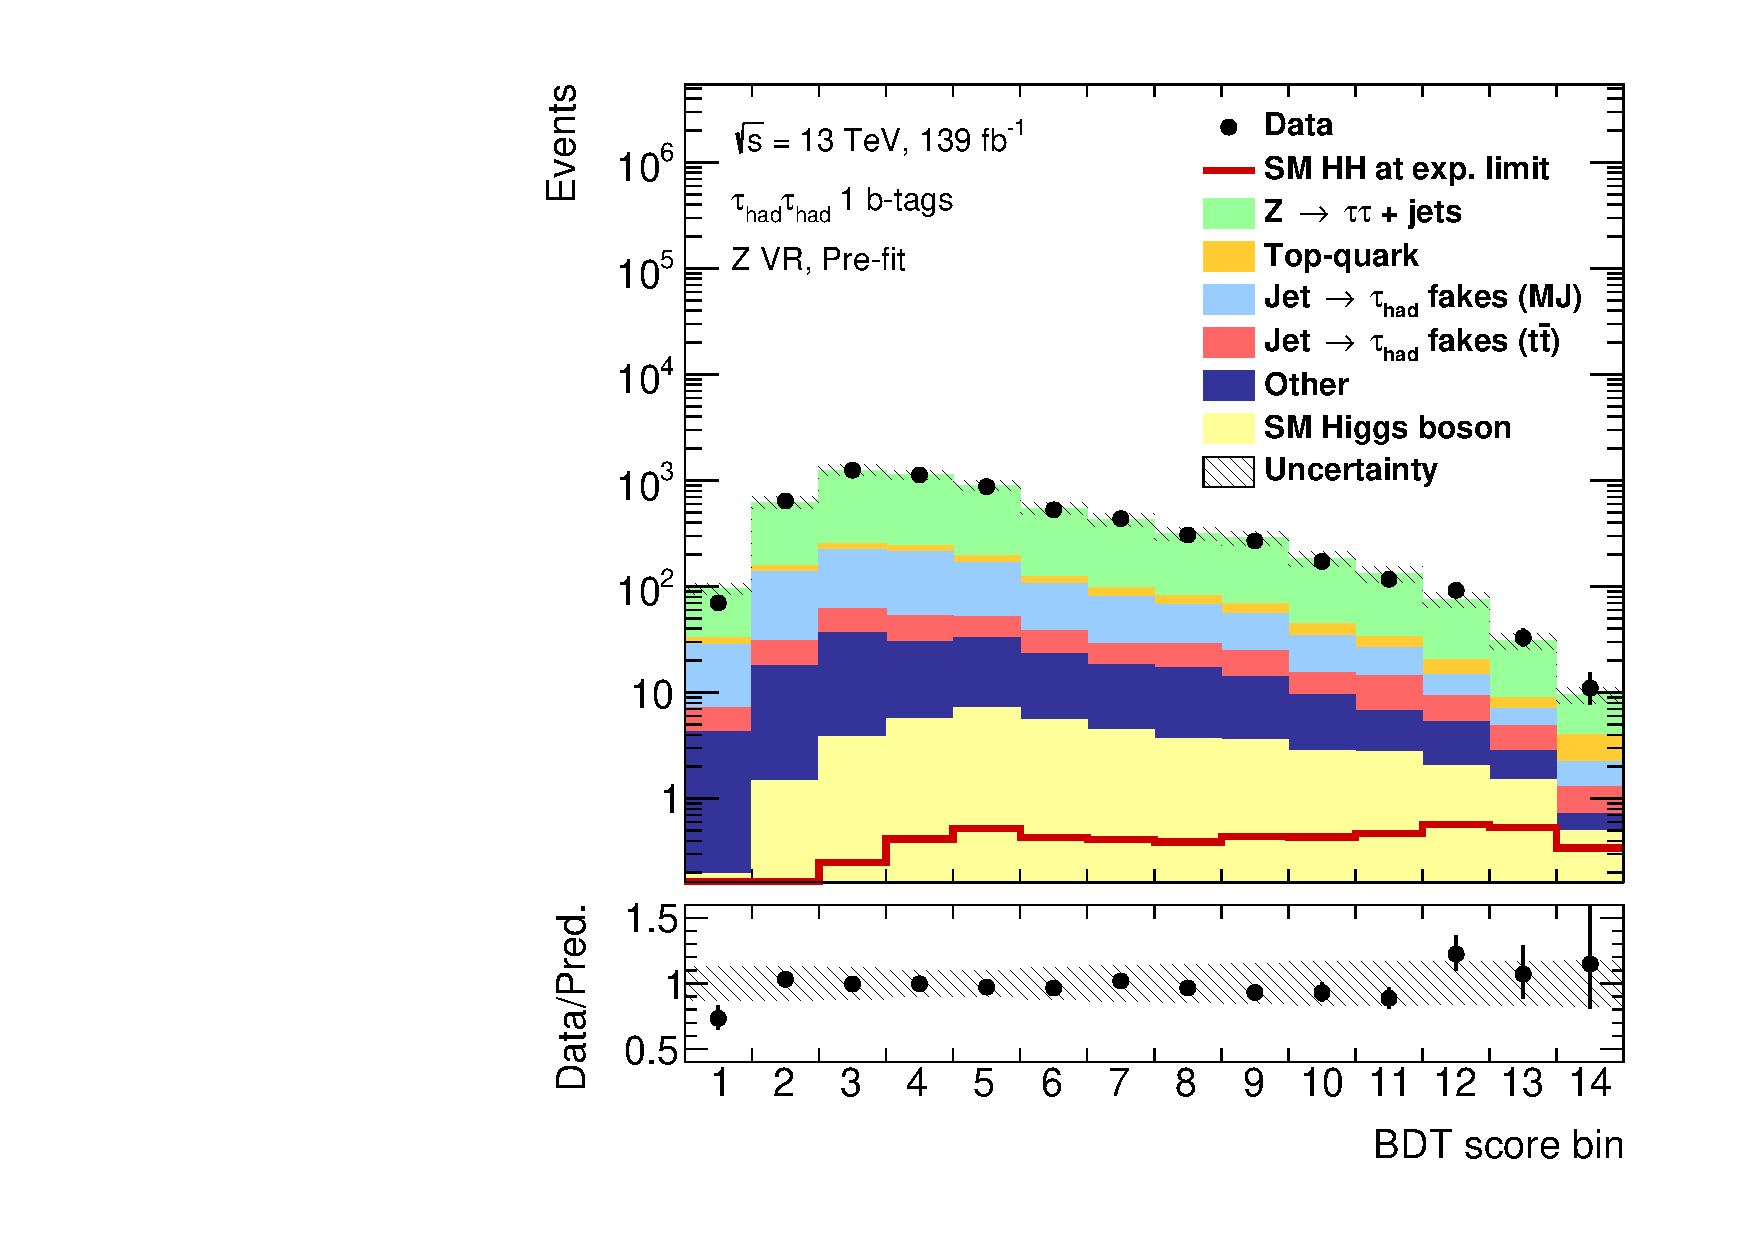
\includegraphics[width=\textwidth]{vrplots/zvr/Region_BMin0_incJet1_distSMBDT_J2_Y2015_DLLOS_T1_SpcTauHH_L0_Prefitlog}
    \subcaption{}
  \end{subfigure}\hfill%
  \begin{subfigure}{0.495\textwidth}
    \centering

    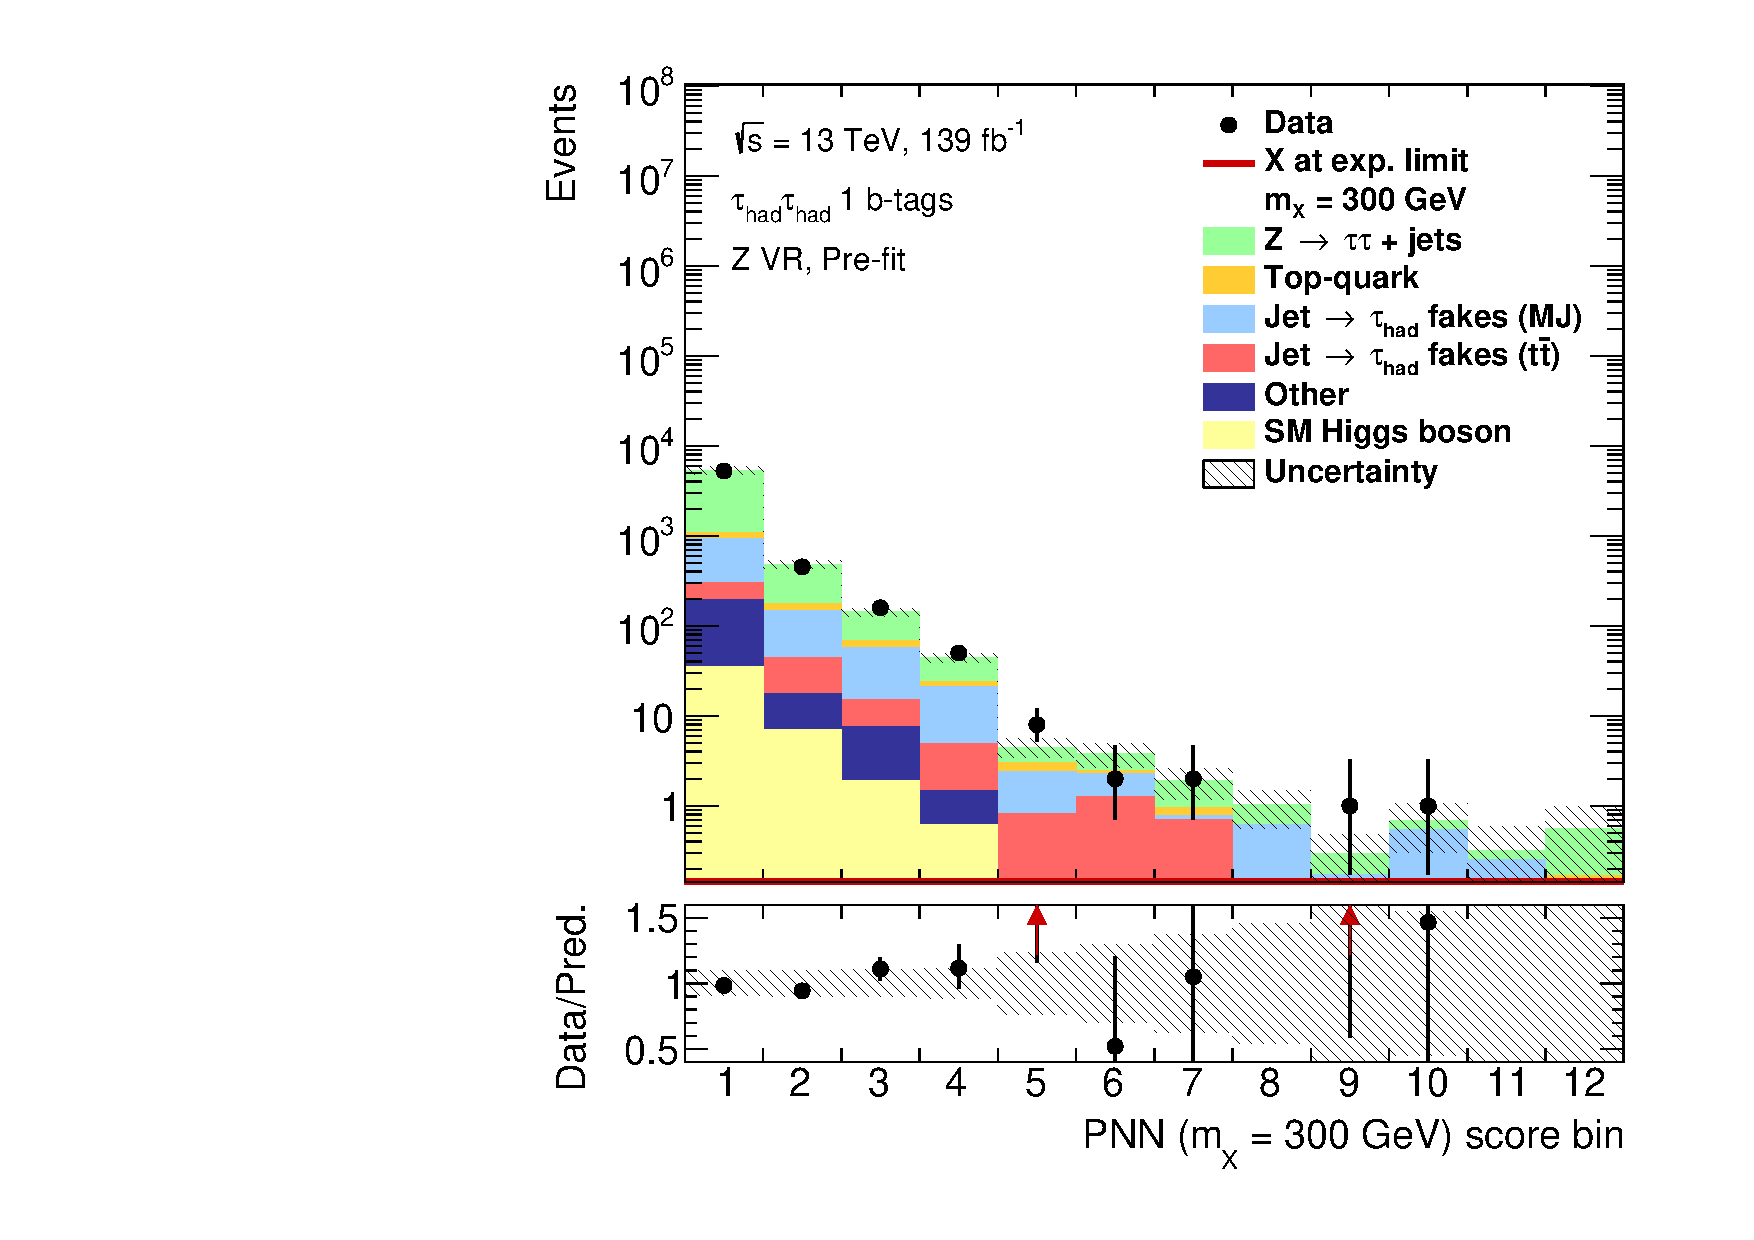
\includegraphics[width=\textwidth]{vrplots/zvr/Region_BMin0_incJet1_distPNN300_J2_Y2015_DLLOS_T1_SpcTauHH_L0_Prefitlog}
    \subcaption{}
  \end{subfigure}

  \begin{subfigure}{0.495\textwidth}
    \centering

    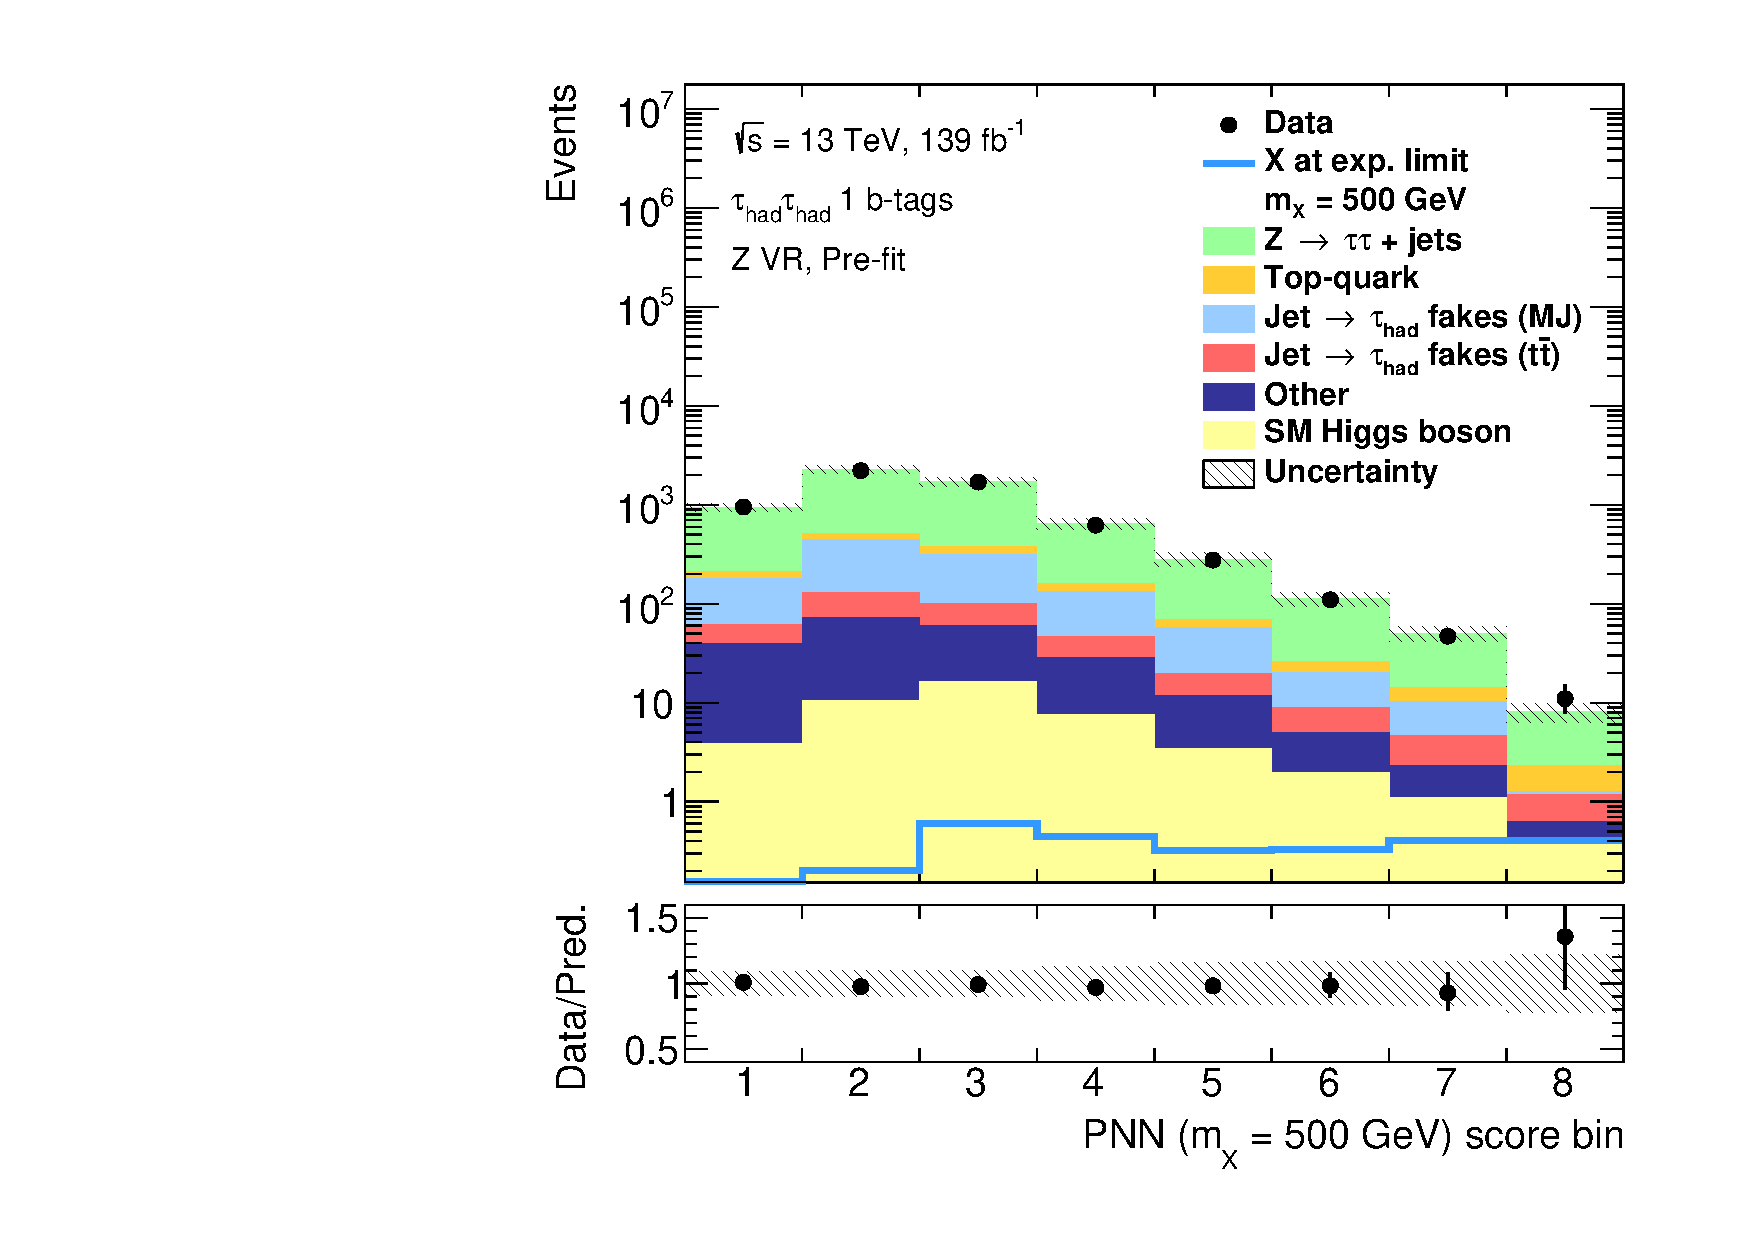
\includegraphics[width=\textwidth]{vrplots/zvr/Region_BMin0_incJet1_distPNN500_J2_Y2015_DLLOS_T1_SpcTauHH_L0_Prefitlog}
    \subcaption{}
  \end{subfigure}\hfill%
  \begin{subfigure}{0.495\textwidth}
    \centering

    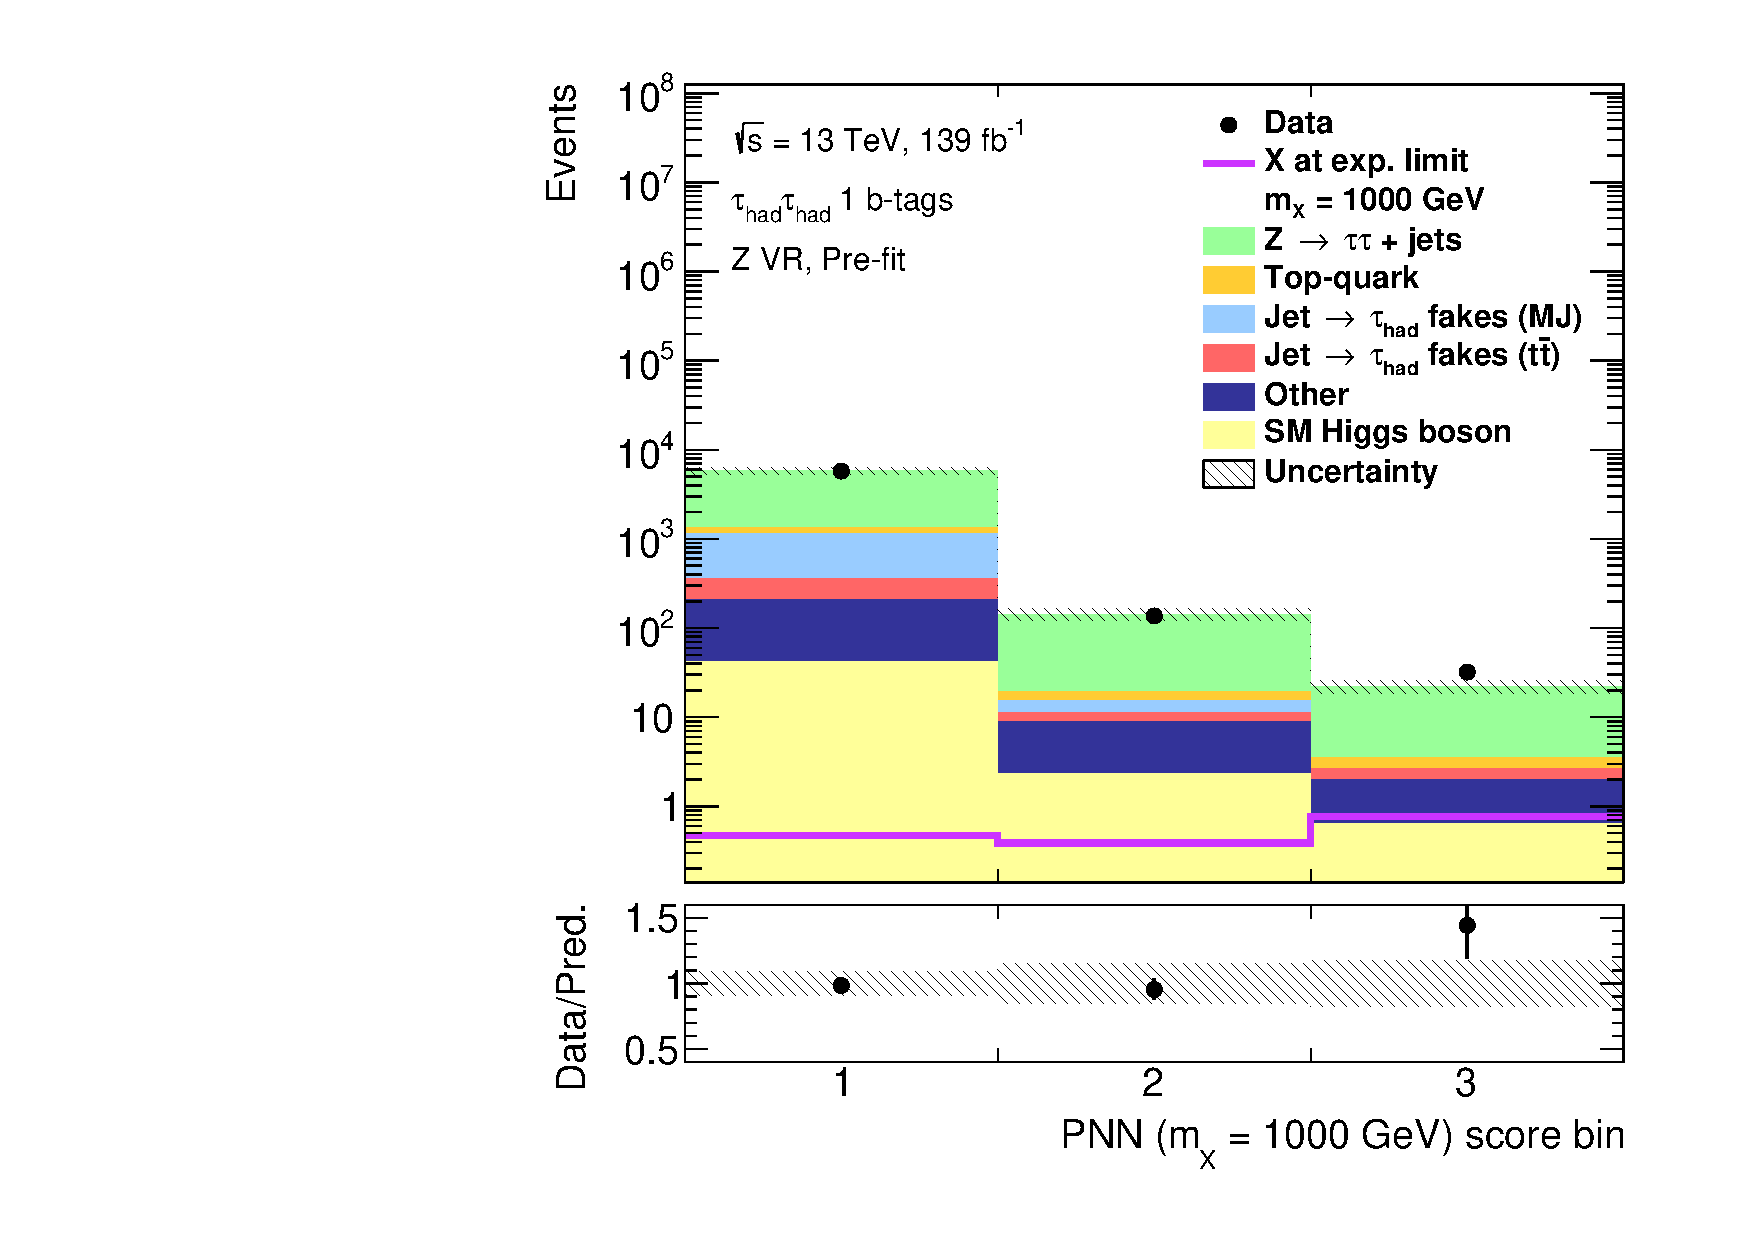
\includegraphics[width=\textwidth]{vrplots/zvr/Region_BMin0_incJet1_distPNN1000_J2_Y2015_DLLOS_T1_SpcTauHH_L0_Prefitlog}
    \subcaption{}
  \end{subfigure}

  \captionof{figure}[BDT and PNN distributions in the \Zjets VR of the \hadhad
  channel prior to the fit.]{BDT (a) and PNN (b-d) distributions in the \Zjets
    VR of the \hadhad channel prior to the fit. The \Zjets VR is defined by
    requiring exactly 1~$b$-tagged jet,
    $\SI{70}{\GeV} < \mMMC < \SI{110}{\GeV}$, and
    $\dRtautau < \SI{0.015}{\per\GeV} \cdot \mMMC + 0.06$. The signals are
    normalised to the expected upper limit for the combination of all channels.}
}


\clearpage
\subsection*{MVA Scores in the SS Control Region}

{
  \centering

  \vspace*{1em}

  \setcaptiontype{figure}

  \begin{subfigure}{0.495\textwidth}
    \centering

    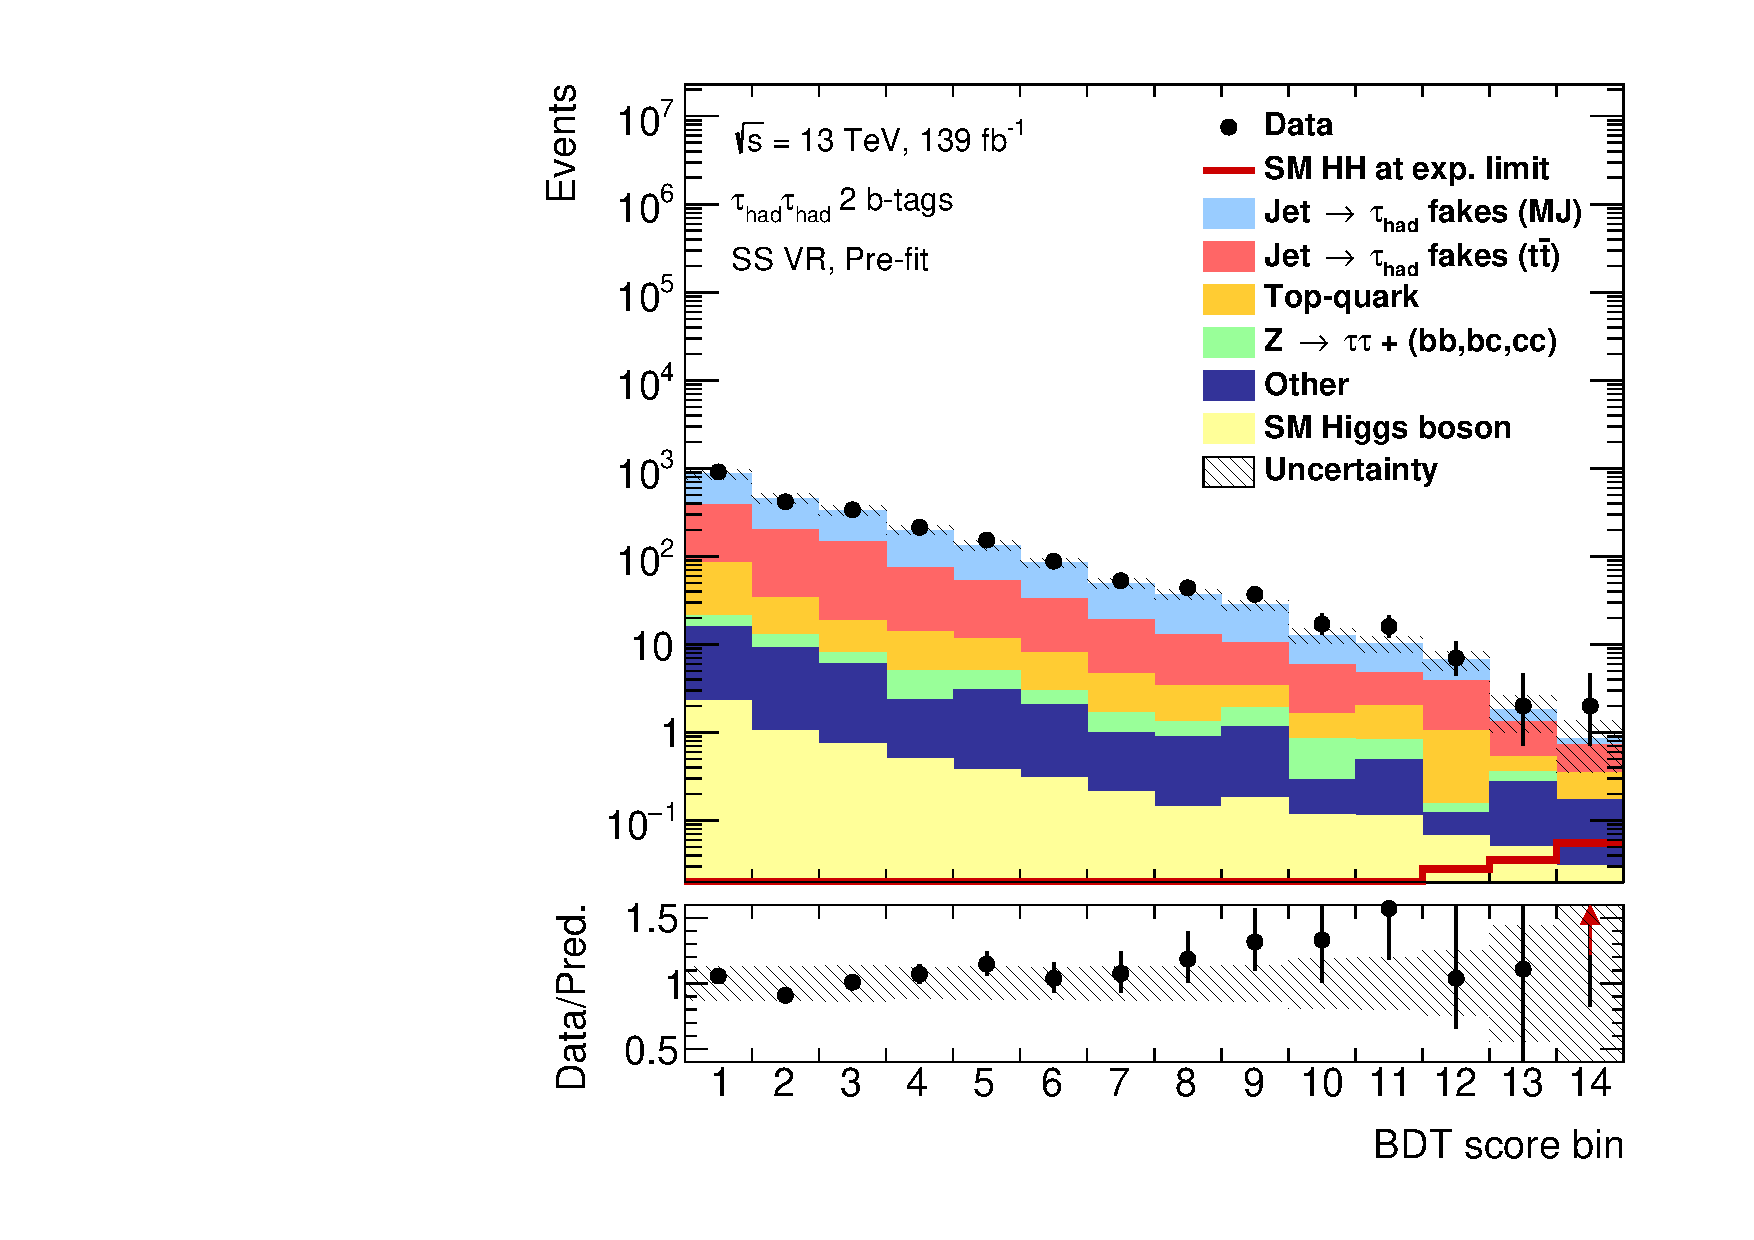
\includegraphics[width=\textwidth]{vrplots/ssvr/Region_BMin0_incJet1_distSMBDT_J2_Y2015_DLLSS_T2_SpcTauHH_L0_Prefitlog}
    \subcaption{}
  \end{subfigure}\hfill%
  \begin{subfigure}{0.495\textwidth}
    \centering

    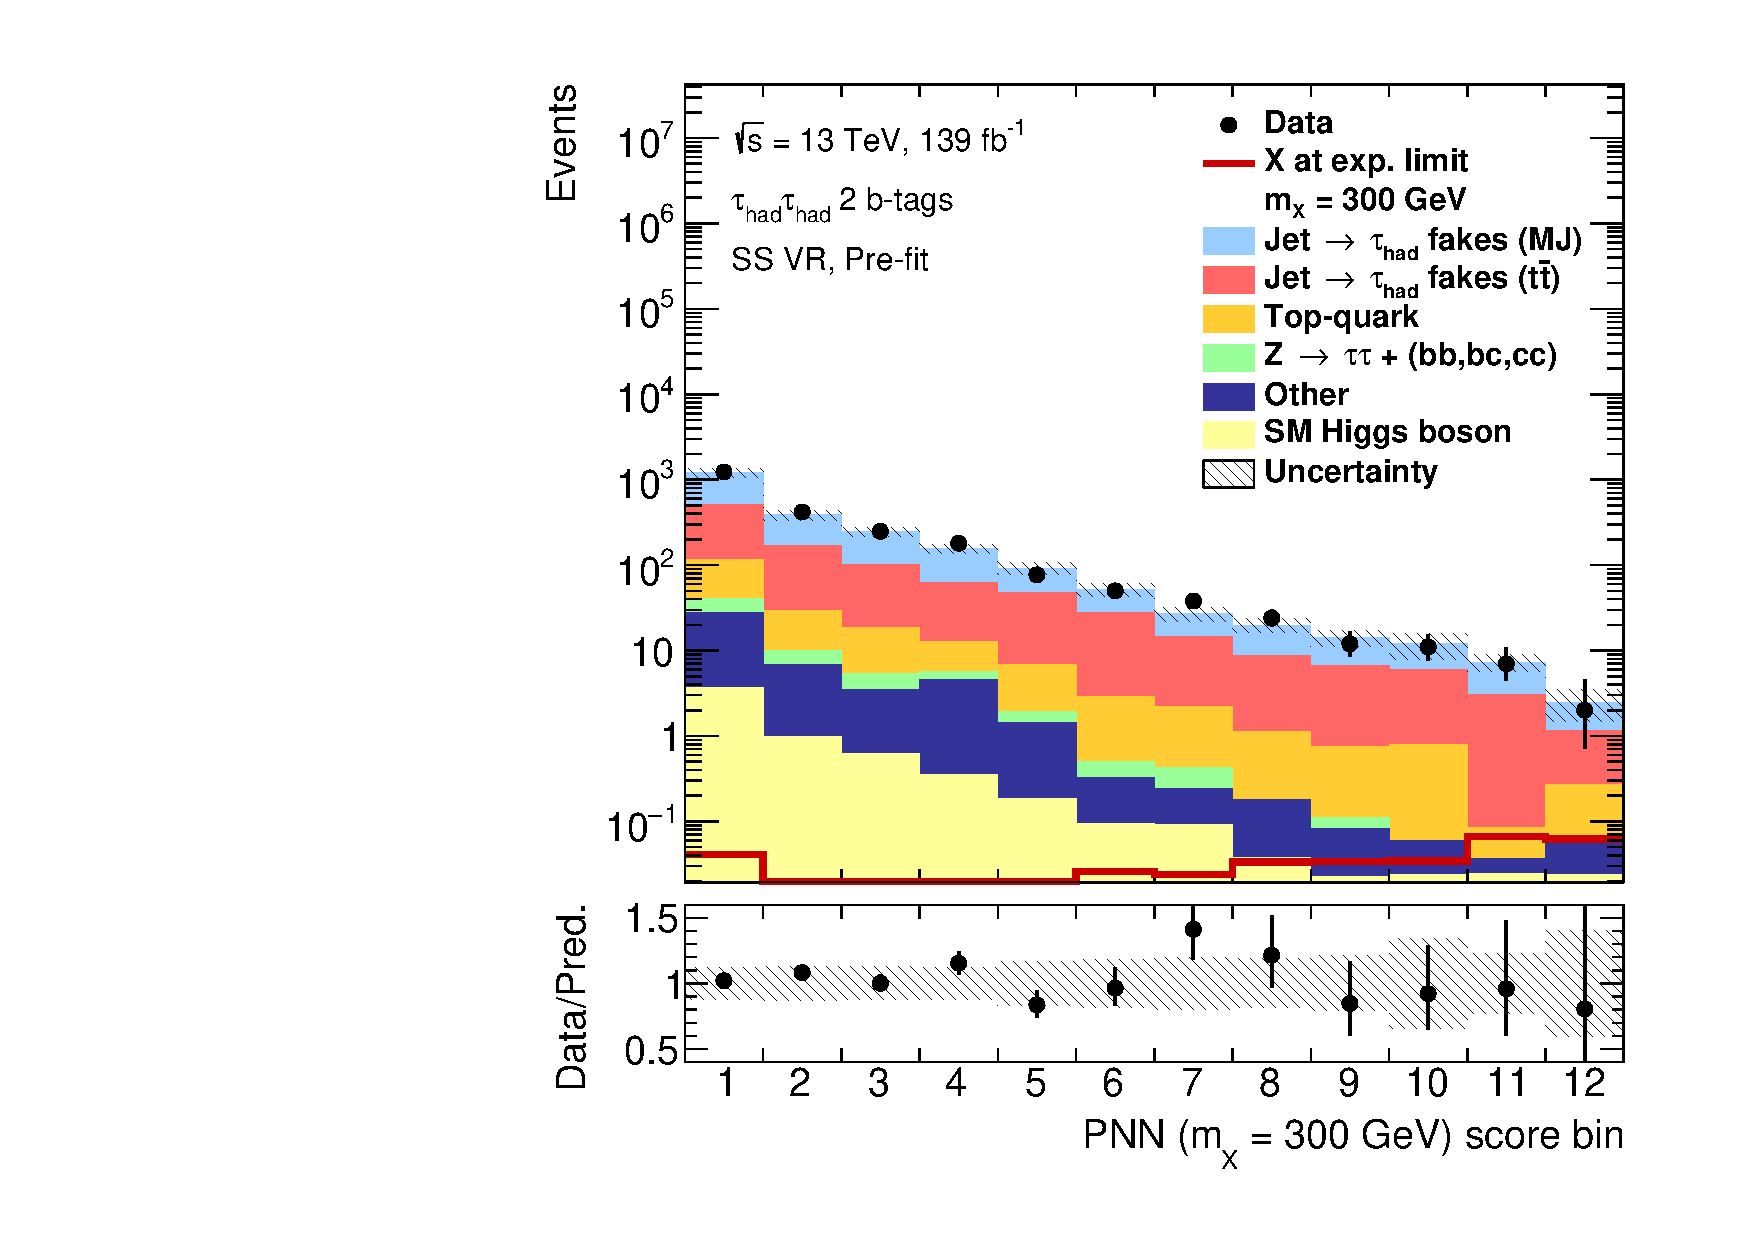
\includegraphics[width=\textwidth]{vrplots/ssvr/Region_BMin0_incJet1_distPNN300_J2_Y2015_DLLSS_T2_SpcTauHH_L0_Prefitlog}
    \subcaption{}
  \end{subfigure}

  \begin{subfigure}{0.495\textwidth}
    \centering

    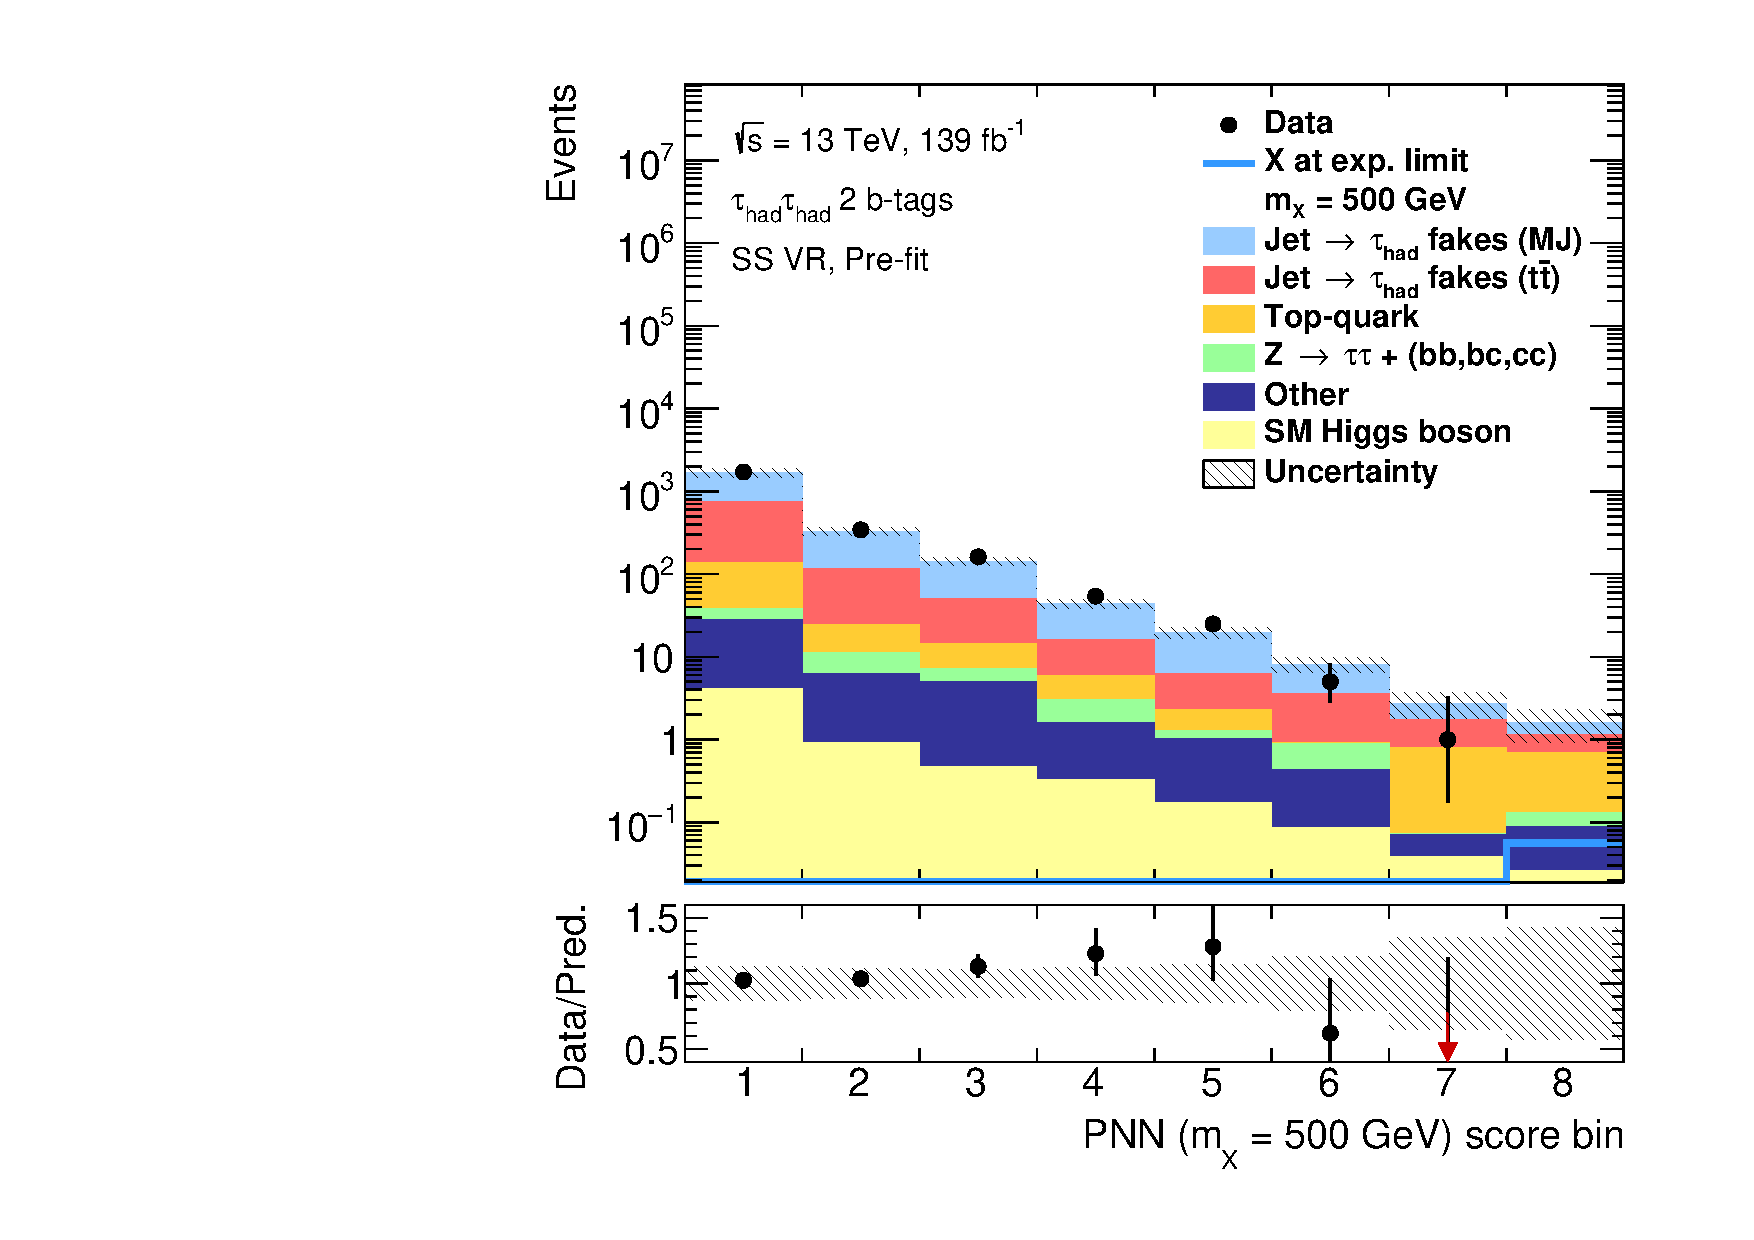
\includegraphics[width=\textwidth]{vrplots/ssvr/Region_BMin0_incJet1_distPNN500_J2_Y2015_DLLSS_T2_SpcTauHH_L0_Prefitlog}
    \subcaption{}
  \end{subfigure}\hfill%
  \begin{subfigure}{0.495\textwidth}
    \centering

    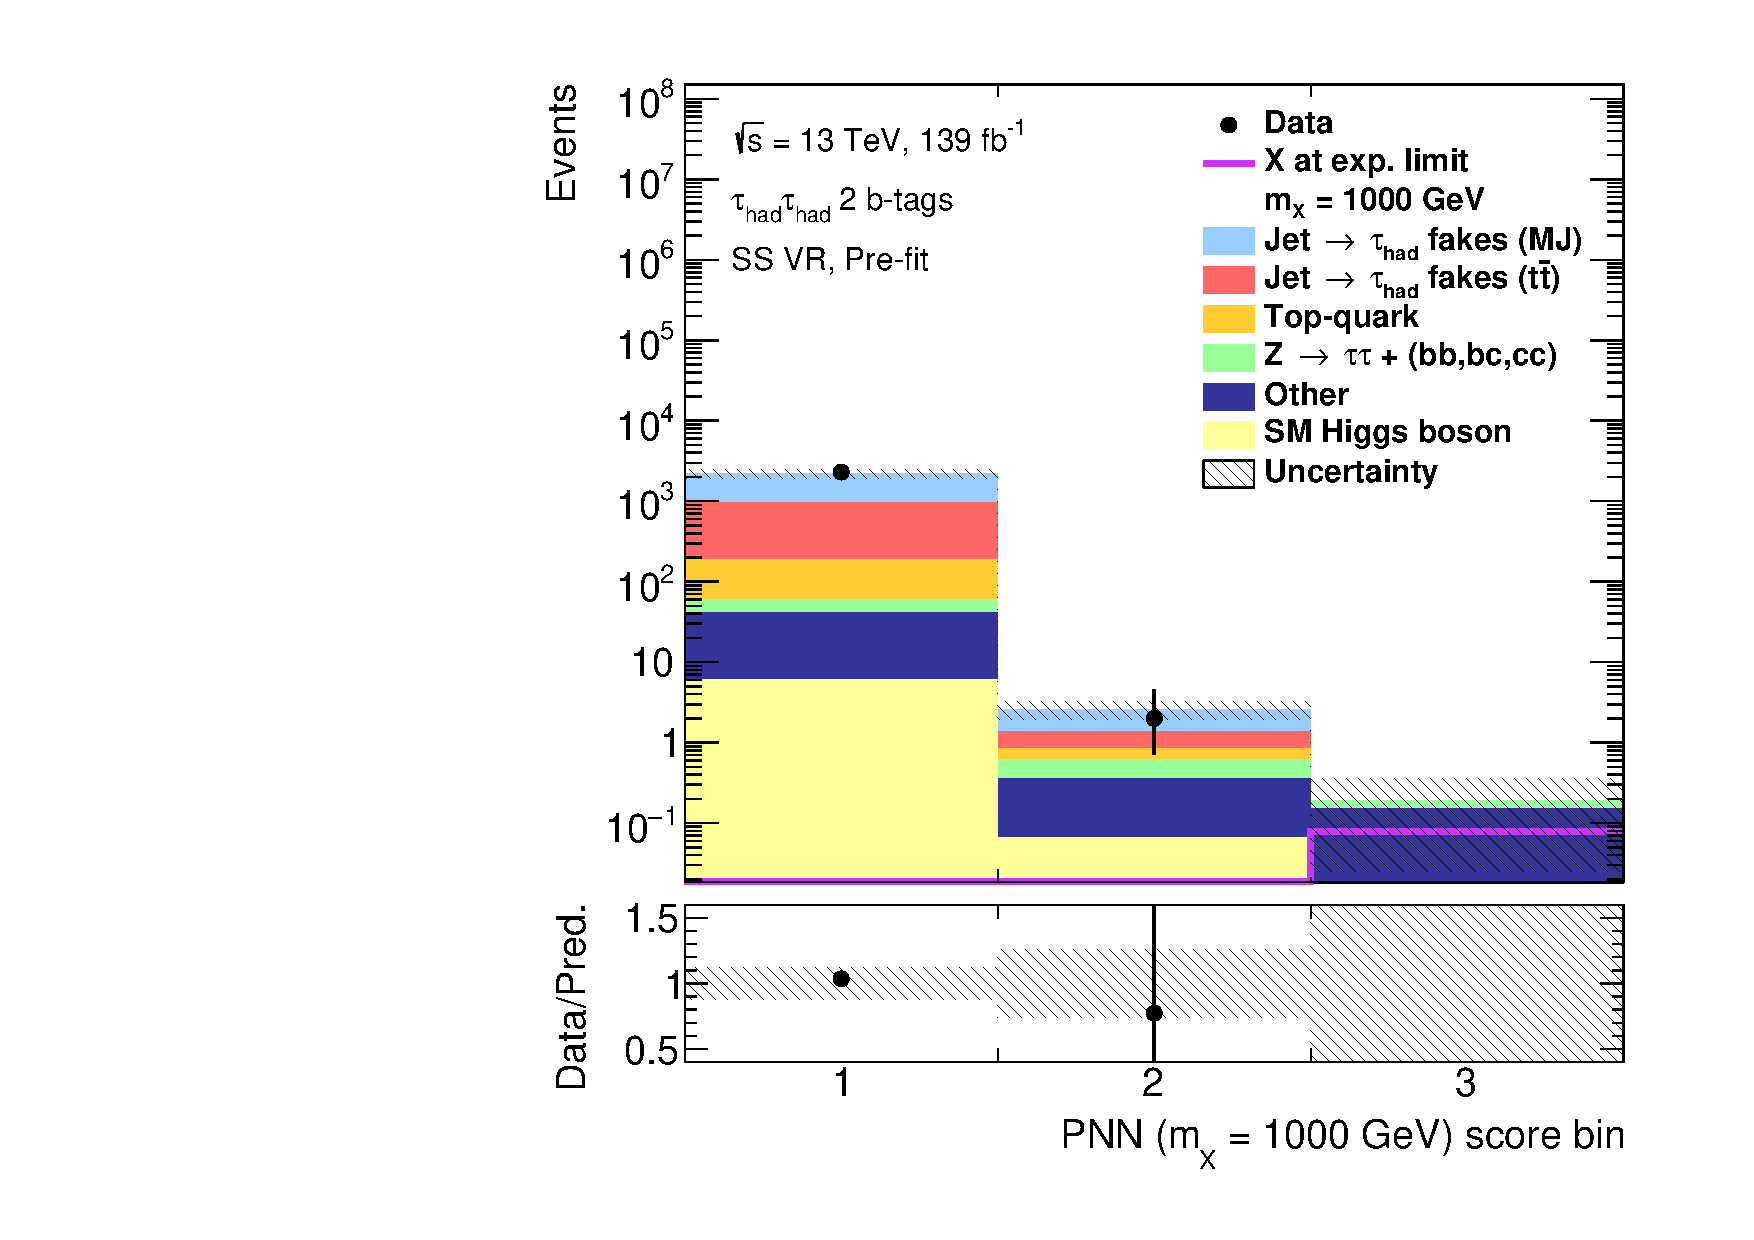
\includegraphics[width=\textwidth]{vrplots/ssvr/Region_BMin0_incJet1_distPNN1000_J2_Y2015_DLLSS_T2_SpcTauHH_L0_Prefitlog}
    \subcaption{}
  \end{subfigure}

  \captionof{figure}[BDT and PNN distributions in the SS~CR of the \hadhad
  channel prior to the fit.]{BDT (a) and PNN (b-d) distributions in the SS~CR of
    the \hadhad channel prior to the fit. The SS~CR is defined by the SR event
    selection but requiring \tauhadvis candidates with electric charges of the
    same sign. The signals are normalised to the expected upper limit for the
    combination of all channels.}
}


%%% Local Variables:
%%% mode: latex
%%% TeX-master: "../../phd_thesis"
%%% End:
